\documentclass[1p]{elsarticle_modified}
%\bibliographystyle{elsarticle-num}

%\usepackage[colorlinks]{hyperref}
%\usepackage{abbrmath_seonhwa} %\Abb, \Ascr, \Acal ,\Abf, \Afrak
\usepackage{amsfonts}
\usepackage{amssymb}
\usepackage{amsmath}
\usepackage{amsthm}
\usepackage{scalefnt}
\usepackage{amsbsy}
\usepackage{kotex}
\usepackage{caption}
\usepackage{subfig}
\usepackage{color}
\usepackage{graphicx}
\usepackage{xcolor} %% white, black, red, green, blue, cyan, magenta, yellow
\usepackage{float}
\usepackage{setspace}
\usepackage{hyperref}

\usepackage{tikz}
\usetikzlibrary{arrows}

\usepackage{multirow}
\usepackage{array} % fixed length table
\usepackage{hhline}

%%%%%%%%%%%%%%%%%%%%%
\makeatletter
\renewcommand*\env@matrix[1][\arraystretch]{%
	\edef\arraystretch{#1}%
	\hskip -\arraycolsep
	\let\@ifnextchar\new@ifnextchar
	\array{*\c@MaxMatrixCols c}}
\makeatother %https://tex.stackexchange.com/questions/14071/how-can-i-increase-the-line-spacing-in-a-matrix
%%%%%%%%%%%%%%%

\usepackage[normalem]{ulem}

\newcommand{\msout}[1]{\ifmmode\text{\sout{\ensuremath{#1}}}\else\sout{#1}\fi}
%SOURCE: \msout is \stkout macro in https://tex.stackexchange.com/questions/20609/strikeout-in-math-mode

\newcommand{\cancel}[1]{
	\ifmmode
	{\color{red}\msout{#1}}
	\else
	{\color{red}\sout{#1}}
	\fi
}

\newcommand{\add}[1]{
	{\color{blue}\uwave{#1}}
}

\newcommand{\replace}[2]{
	\ifmmode
	{\color{red}\msout{#1}}{\color{blue}\uwave{#2}}
	\else
	{\color{red}\sout{#1}}{\color{blue}\uwave{#2}}
	\fi
}

\newcommand{\Sol}{\mathcal{S}} %segment
\newcommand{\D}{D} %diagram
\newcommand{\A}{\mathcal{A}} %arc


%%%%%%%%%%%%%%%%%%%%%%%%%%%%%5 test

\def\sl{\operatorname{\textup{SL}}(2,\Cbb)}
\def\psl{\operatorname{\textup{PSL}}(2,\Cbb)}
\def\quan{\mkern 1mu \triangleright \mkern 1mu}

\theoremstyle{definition}
\newtheorem{thm}{Theorem}[section]
\newtheorem{prop}[thm]{Proposition}
\newtheorem{lem}[thm]{Lemma}
\newtheorem{ques}[thm]{Question}
\newtheorem{cor}[thm]{Corollary}
\newtheorem{defn}[thm]{Definition}
\newtheorem{exam}[thm]{Example}
\newtheorem{rmk}[thm]{Remark}
\newtheorem{alg}[thm]{Algorithm}

\newcommand{\I}{\sqrt{-1}}
\begin{document}

%\begin{frontmatter}
%
%\title{Boundary parabolic representations of knots up to 8 crossings}
%
%%% Group authors per affiliation:
%\author{Yunhi Cho} 
%\address{Department of Mathematics, University of Seoul, Seoul, Korea}
%\ead{yhcho@uos.ac.kr}
%
%
%\author{Seonhwa Kim} %\fnref{s_kim}}
%\address{Center for Geometry and Physics, Institute for Basic Science, Pohang, 37673, Korea}
%\ead{ryeona17@ibs.re.kr}
%
%\author{Hyuk Kim}
%\address{Department of Mathematical Sciences, Seoul National University, Seoul 08826, Korea}
%\ead{hyukkim@snu.ac.kr}
%
%\author{Seokbeom Yoon}
%\address{Department of Mathematical Sciences, Seoul National University, Seoul, 08826,  Korea}
%\ead{sbyoon15@snu.ac.kr}
%
%\begin{abstract}
%We find all boundary parabolic representation of knots up to 8 crossings.
%
%\end{abstract}
%\begin{keyword}
%    \MSC[2010] 57M25 
%\end{keyword}
%
%\end{frontmatter}

%\linenumbers
%\tableofcontents
%
\newcommand\colored[1]{\textcolor{white}{\rule[-0.35ex]{0.8em}{1.4ex}}\kern-0.8em\color{red} #1}%
%\newcommand\colored[1]{\textcolor{white}{ #1}\kern-2.17ex	\textcolor{white}{ #1}\kern-1.81ex	\textcolor{white}{ #1}\kern-2.15ex\color{red}#1	}

{\Large $\underline{12a_{0123}~(K12a_{0123})}$}

\setlength{\tabcolsep}{10pt}
\renewcommand{\arraystretch}{1.6}
\vspace{1cm}\begin{tabular}{m{100pt}>{\centering\arraybackslash}m{274pt}}
\multirow{5}{120pt}{
	\centering
	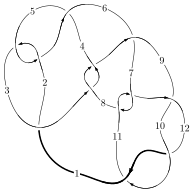
\includegraphics[width=112pt]{../../../GIT/diagram.site/Diagrams/png/924_12a_0123.png}\\
\ \ \ A knot diagram\footnotemark}&
\allowdisplaybreaks
\textbf{Linearized knot diagam} \\
\cline{2-2}
 &
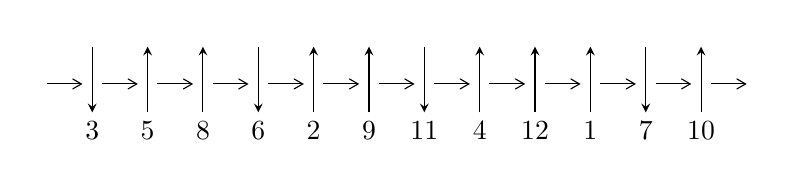
\begin{tikzpicture}[x=20pt, y=17pt]
	% nodes
	\node (C0) at (0, 0) {};
	\node (C1) at (1, 0) {};
	\node (C1U) at (1, +1) {};
	\node (C1D) at (1, -1) {3};

	\node (C2) at (2, 0) {};
	\node (C2U) at (2, +1) {};
	\node (C2D) at (2, -1) {5};

	\node (C3) at (3, 0) {};
	\node (C3U) at (3, +1) {};
	\node (C3D) at (3, -1) {8};

	\node (C4) at (4, 0) {};
	\node (C4U) at (4, +1) {};
	\node (C4D) at (4, -1) {6};

	\node (C5) at (5, 0) {};
	\node (C5U) at (5, +1) {};
	\node (C5D) at (5, -1) {2};

	\node (C6) at (6, 0) {};
	\node (C6U) at (6, +1) {};
	\node (C6D) at (6, -1) {9};

	\node (C7) at (7, 0) {};
	\node (C7U) at (7, +1) {};
	\node (C7D) at (7, -1) {11};

	\node (C8) at (8, 0) {};
	\node (C8U) at (8, +1) {};
	\node (C8D) at (8, -1) {4};

	\node (C9) at (9, 0) {};
	\node (C9U) at (9, +1) {};
	\node (C9D) at (9, -1) {12};

	\node (C10) at (10, 0) {};
	\node (C10U) at (10, +1) {};
	\node (C10D) at (10, -1) {1};

	\node (C11) at (11, 0) {};
	\node (C11U) at (11, +1) {};
	\node (C11D) at (11, -1) {7};

	\node (C12) at (12, 0) {};
	\node (C12U) at (12, +1) {};
	\node (C12D) at (12, -1) {10};
	\node (C13) at (13, 0) {};

	% arrows
	\draw[->,>={angle 60}]
	(C0) edge (C1) (C1) edge (C2) (C2) edge (C3) (C3) edge (C4) (C4) edge (C5) (C5) edge (C6) (C6) edge (C7) (C7) edge (C8) (C8) edge (C9) (C9) edge (C10) (C10) edge (C11) (C11) edge (C12) (C12) edge (C13) ;	\draw[->,>=stealth]
	(C1U) edge (C1D) (C2D) edge (C2U) (C3D) edge (C3U) (C4U) edge (C4D) (C5D) edge (C5U) (C6D) edge (C6U) (C7U) edge (C7D) (C8D) edge (C8U) (C9D) edge (C9U) (C10D) edge (C10U) (C11U) edge (C11D) (C12D) edge (C12U) ;
	\end{tikzpicture} \\
\hhline{~~} \\& 
\textbf{Solving Sequence} \\ \cline{2-2} 
 &
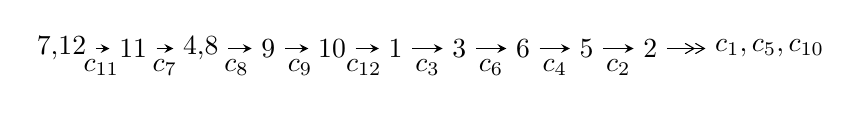
\begin{tikzpicture}[x=23pt, y=7pt]
	% node
	\node (A0) at (-1/8, 0) {7,12};
	\node (A1) at (1, 0) {11};
	\node (A2) at (33/16, 0) {4,8};
	\node (A3) at (25/8, 0) {9};
	\node (A4) at (33/8, 0) {10};
	\node (A5) at (41/8, 0) {1};
	\node (A6) at (49/8, 0) {3};
	\node (A7) at (57/8, 0) {6};
	\node (A8) at (65/8, 0) {5};
	\node (A9) at (73/8, 0) {2};
	\node (C1) at (1/2, -1) {$c_{11}$};
	\node (C2) at (3/2, -1) {$c_{7}$};
	\node (C3) at (21/8, -1) {$c_{8}$};
	\node (C4) at (29/8, -1) {$c_{9}$};
	\node (C5) at (37/8, -1) {$c_{12}$};
	\node (C6) at (45/8, -1) {$c_{3}$};
	\node (C7) at (53/8, -1) {$c_{6}$};
	\node (C8) at (61/8, -1) {$c_{4}$};
	\node (C9) at (69/8, -1) {$c_{2}$};
	\node (A10) at (11, 0) {$c_{1},c_{5},c_{10}$};

	% edge
	\draw[->,>=stealth]	
	(A0) edge (A1) (A1) edge (A2) (A2) edge (A3) (A3) edge (A4) (A4) edge (A5) (A5) edge (A6) (A6) edge (A7) (A7) edge (A8) (A8) edge (A9) ;
	\draw[->>,>={angle 60}]	
	(A9) edge (A10);
\end{tikzpicture} \\ 

\end{tabular} \\

\footnotetext{
The image of knot diagram is generated by the software ``\textbf{Draw programme}" developed by Andrew Bartholomew(\url{http://www.layer8.co.uk/maths/draw/index.htm\#Running-draw}), where we modified some parts for our purpose(\url{https://github.com/CATsTAILs/LinksPainter}).
}\phantom \\ \newline 
\centering \textbf{Ideals for irreducible components\footnotemark of $X_{\text{par}}$} 
 
\begin{align*}
I^u_{1}&=\langle 
2.51942\times10^{285} u^{92}+8.00642\times10^{285} u^{91}+\cdots+4.40333\times10^{288} b-5.99526\times10^{288},\\
\phantom{I^u_{1}}&\phantom{= \langle  }3.85027\times10^{286} u^{92}+1.46536\times10^{287} u^{91}+\cdots+8.80666\times10^{288} a-6.43241\times10^{289},\\
\phantom{I^u_{1}}&\phantom{= \langle  }u^{93}+3 u^{92}+\cdots-1024 u+512\rangle \\
I^u_{2}&=\langle 
u^2 a+b+a,\;- u^4 a+u^3 a+u^4-2 u^2 a+a^2+a u+u^2- a+u,\;u^5- u^4+2 u^3- u^2+u-1\rangle \\
\\
I^v_{1}&=\langle 
a,\;v^8+4 v^7+7 v^6+4 v^5-3 v^4-6 v^3-2 v^2+b+1,\;v^9+5 v^8+12 v^7+15 v^6+9 v^5- v^4-4 v^3-2 v^2+v+1\rangle \\
\end{align*}
\raggedright * 3 irreducible components of $\dim_{\mathbb{C}}=0$, with total 112 representations.\\
\footnotetext{All coefficients of polynomials are rational numbers. But the coefficients are sometimes approximated in decimal forms when there is not enough margin.}
\newpage
\renewcommand{\arraystretch}{1}
\centering \section*{I. $I^u_{1}= \langle 2.52\times10^{285} u^{92}+8.01\times10^{285} u^{91}+\cdots+4.40\times10^{288} b-6.00\times10^{288},\;3.85\times10^{286} u^{92}+1.47\times10^{287} u^{91}+\cdots+8.81\times10^{288} a-6.43\times10^{289},\;u^{93}+3 u^{92}+\cdots-1024 u+512 \rangle$}
\flushleft \textbf{(i) Arc colorings}\\
\begin{tabular}{m{7pt} m{180pt} m{7pt} m{180pt} }
\flushright $a_{7}=$&$\begin{pmatrix}0\\u\end{pmatrix}$ \\
\flushright $a_{12}=$&$\begin{pmatrix}1\\0\end{pmatrix}$ \\
\flushright $a_{11}=$&$\begin{pmatrix}1\\- u^2\end{pmatrix}$ \\
\flushright $a_{4}=$&$\begin{pmatrix}-0.00437199 u^{92}-0.0166393 u^{91}+\cdots+5.57776 u+7.30402\\-0.000572162 u^{92}-0.00181826 u^{91}+\cdots-0.396111 u+1.36153\end{pmatrix}$ \\
\flushright $a_{8}=$&$\begin{pmatrix}- u\\u^3+u\end{pmatrix}$ \\
\flushright $a_{9}=$&$\begin{pmatrix}-0.0121780 u^{92}-0.0398559 u^{91}+\cdots-3.82371 u+10.7352\\0.00336113 u^{92}+0.0126239 u^{91}+\cdots-0.559837 u-5.16081\end{pmatrix}$ \\
\flushright $a_{10}=$&$\begin{pmatrix}-0.00881684 u^{92}-0.0272320 u^{91}+\cdots-4.38355 u+5.57440\\0.00336113 u^{92}+0.0126239 u^{91}+\cdots-0.559837 u-5.16081\end{pmatrix}$ \\
\flushright $a_{1}=$&$\begin{pmatrix}-0.00881684 u^{92}-0.0272320 u^{91}+\cdots-4.38355 u+5.57440\\-0.00804363 u^{92}-0.0257825 u^{91}+\cdots-3.15420 u+4.76072\end{pmatrix}$ \\
\flushright $a_{3}=$&$\begin{pmatrix}-0.000573324 u^{92}-0.00638541 u^{91}+\cdots+8.37452 u+3.38703\\-0.00392517 u^{92}-0.0143906 u^{91}+\cdots-0.0783778 u+4.69374\end{pmatrix}$ \\
\flushright $a_{6}=$&$\begin{pmatrix}0.00770029 u^{92}+0.0301959 u^{91}+\cdots-2.38268 u-3.55915\\0.000870195 u^{92}+0.00510555 u^{91}+\cdots+0.0219210 u+0.395882\end{pmatrix}$ \\
\flushright $a_{5}=$&$\begin{pmatrix}-0.00441454 u^{92}-0.0207171 u^{91}+\cdots+8.92302 u+2.84951\\-0.00237340 u^{92}-0.00983384 u^{91}+\cdots-1.33682 u+1.89139\end{pmatrix}$ \\
\flushright $a_{2}=$&$\begin{pmatrix}-0.00236713 u^{92}-0.00962072 u^{91}+\cdots+4.13460 u-0.151447\\-0.00720868 u^{92}-0.0248131 u^{91}+\cdots-3.72884 u+5.65750\end{pmatrix}$\\&\end{tabular}
\flushleft \textbf{(ii) Obstruction class $= -1$}\\~\\
\flushleft \textbf{(iii) Cusp Shapes $= -0.0147962 u^{92}-0.0552504 u^{91}+\cdots+35.4620 u+14.3294$}\\~\\
\newpage\renewcommand{\arraystretch}{1}
\flushleft \textbf{(iv) u-Polynomials at the component}\newline \\
\begin{tabular}{m{50pt}|m{274pt}}
Crossings & \hspace{64pt}u-Polynomials at each crossing \\
\hline $$\begin{aligned}c_{1},c_{4}\end{aligned}$$&$\begin{aligned}
&u^{93}+29 u^{92}+\cdots+3 u-1
\end{aligned}$\\
\hline $$\begin{aligned}c_{2},c_{5}\end{aligned}$$&$\begin{aligned}
&u^{93}+7 u^{92}+\cdots+3 u-1
\end{aligned}$\\
\hline $$\begin{aligned}c_{3},c_{8}\end{aligned}$$&$\begin{aligned}
&u^{93}-2 u^{92}+\cdots-4096 u+1024
\end{aligned}$\\
\hline $$\begin{aligned}c_{6}\end{aligned}$$&$\begin{aligned}
&u^{93}+4 u^{92}+\cdots+7544 u+1681
\end{aligned}$\\
\hline $$\begin{aligned}c_{7},c_{11}\end{aligned}$$&$\begin{aligned}
&u^{93}+3 u^{92}+\cdots-1024 u+512
\end{aligned}$\\
\hline $$\begin{aligned}c_{9},c_{10},c_{12}\end{aligned}$$&$\begin{aligned}
&u^{93}+12 u^{92}+\cdots+6 u+1
\end{aligned}$\\
\hline
\end{tabular}\\~\\
\newpage\renewcommand{\arraystretch}{1}
\flushleft \textbf{(v) Riley Polynomials at the component}\newline \\
\begin{tabular}{m{50pt}|m{274pt}}
Crossings & \hspace{64pt}Riley Polynomials at each crossing \\
\hline $$\begin{aligned}c_{1},c_{4}\end{aligned}$$&$\begin{aligned}
&y^{93}+77 y^{92}+\cdots+1907 y-1
\end{aligned}$\\
\hline $$\begin{aligned}c_{2},c_{5}\end{aligned}$$&$\begin{aligned}
&y^{93}+29 y^{92}+\cdots+3 y-1
\end{aligned}$\\
\hline $$\begin{aligned}c_{3},c_{8}\end{aligned}$$&$\begin{aligned}
&y^{93}-60 y^{92}+\cdots+10485760 y-1048576
\end{aligned}$\\
\hline $$\begin{aligned}c_{6}\end{aligned}$$&$\begin{aligned}
&y^{93}-62 y^{92}+\cdots-79232254 y-2825761
\end{aligned}$\\
\hline $$\begin{aligned}c_{7},c_{11}\end{aligned}$$&$\begin{aligned}
&y^{93}+63 y^{92}+\cdots+1048576 y-262144
\end{aligned}$\\
\hline $$\begin{aligned}c_{9},c_{10},c_{12}\end{aligned}$$&$\begin{aligned}
&y^{93}-94 y^{92}+\cdots+46 y-1
\end{aligned}$\\
\hline
\end{tabular}\\~\\
\newpage\flushleft \textbf{(vi) Complex Volumes and Cusp Shapes}
$$\begin{array}{c|c|c}  
\text{Solutions to }I^u_{1}& \I (\text{vol} + \sqrt{-1}CS) & \text{Cusp shape}\\
 \hline 
\begin{aligned}
u &= -0.716646 + 0.701981 I \\
a &= \phantom{-}0.105914 + 0.387753 I \\
b &= \phantom{-}0.124940 + 0.652647 I\end{aligned}
 & \phantom{-}2.16512 + 5.38944 I & \phantom{-0.000000 } 0 \\ \hline\begin{aligned}
u &= -0.716646 - 0.701981 I \\
a &= \phantom{-}0.105914 - 0.387753 I \\
b &= \phantom{-}0.124940 - 0.652647 I\end{aligned}
 & \phantom{-}2.16512 - 5.38944 I & \phantom{-0.000000 } 0 \\ \hline\begin{aligned}
u &= \phantom{-}0.326973 + 0.954295 I \\
a &= \phantom{-}0.619905 + 0.869125 I \\
b &= \phantom{-}0.546397 + 0.505887 I\end{aligned}
 & \phantom{-}6.00254 - 8.25583 I & \phantom{-0.000000 } 0 \\ \hline\begin{aligned}
u &= \phantom{-}0.326973 - 0.954295 I \\
a &= \phantom{-}0.619905 - 0.869125 I \\
b &= \phantom{-}0.546397 - 0.505887 I\end{aligned}
 & \phantom{-}6.00254 + 8.25583 I & \phantom{-0.000000 } 0 \\ \hline\begin{aligned}
u &= -0.684870 + 0.783633 I \\
a &= -0.099146 - 0.337681 I \\
b &= -0.207481 - 0.628643 I\end{aligned}
 & \phantom{-}2.41502 - 0.18063 I & \phantom{-0.000000 } 0 \\ \hline\begin{aligned}
u &= -0.684870 - 0.783633 I \\
a &= -0.099146 + 0.337681 I \\
b &= -0.207481 + 0.628643 I\end{aligned}
 & \phantom{-}2.41502 + 0.18063 I & \phantom{-0.000000 } 0 \\ \hline\begin{aligned}
u &= \phantom{-}0.920090 + 0.240027 I \\
a &= \phantom{-}0.041844 - 0.175746 I \\
b &= -0.504669 + 0.954860 I\end{aligned}
 & \phantom{-}1.78871 + 0.48442 I & \phantom{-0.000000 } 0 \\ \hline\begin{aligned}
u &= \phantom{-}0.920090 - 0.240027 I \\
a &= \phantom{-}0.041844 + 0.175746 I \\
b &= -0.504669 - 0.954860 I\end{aligned}
 & \phantom{-}1.78871 - 0.48442 I & \phantom{-0.000000 } 0 \\ \hline\begin{aligned}
u &= -0.416522 + 0.984253 I \\
a &= -0.108854 - 0.193496 I \\
b &= -0.494465 - 0.255957 I\end{aligned}
 & -0.72672 + 2.38399 I & \phantom{-0.000000 } 0 \\ \hline\begin{aligned}
u &= -0.416522 - 0.984253 I \\
a &= -0.108854 + 0.193496 I \\
b &= -0.494465 + 0.255957 I\end{aligned}
 & -0.72672 - 2.38399 I & \phantom{-0.000000 } 0\\
 \hline 
 \end{array}$$\newpage$$\begin{array}{c|c|c}  
\text{Solutions to }I^u_{1}& \I (\text{vol} + \sqrt{-1}CS) & \text{Cusp shape}\\
 \hline 
\begin{aligned}
u &= \phantom{-}0.106666 + 1.072270 I \\
a &= \phantom{-}1.262650 + 0.357117 I \\
b &= \phantom{-}0.857579 + 0.565640 I\end{aligned}
 & \phantom{-}1.77787 - 2.72179 I & \phantom{-0.000000 } 0 \\ \hline\begin{aligned}
u &= \phantom{-}0.106666 - 1.072270 I \\
a &= \phantom{-}1.262650 - 0.357117 I \\
b &= \phantom{-}0.857579 - 0.565640 I\end{aligned}
 & \phantom{-}1.77787 + 2.72179 I & \phantom{-0.000000 } 0 \\ \hline\begin{aligned}
u &= \phantom{-}0.705042 + 0.824626 I \\
a &= \phantom{-}0.028648 + 0.267284 I \\
b &= \phantom{-}1.12864 - 1.02229 I\end{aligned}
 & \phantom{-}5.76366 + 4.24931 I & \phantom{-0.000000 } 0 \\ \hline\begin{aligned}
u &= \phantom{-}0.705042 - 0.824626 I \\
a &= \phantom{-}0.028648 - 0.267284 I \\
b &= \phantom{-}1.12864 + 1.02229 I\end{aligned}
 & \phantom{-}5.76366 - 4.24931 I & \phantom{-0.000000 } 0 \\ \hline\begin{aligned}
u &= \phantom{-}0.781820 + 0.757204 I \\
a &= -0.012561 - 0.256334 I \\
b &= -1.07841 + 1.07714 I\end{aligned}
 & \phantom{-}5.87081 - 1.54110 I & \phantom{-0.000000 } 0 \\ \hline\begin{aligned}
u &= \phantom{-}0.781820 - 0.757204 I \\
a &= -0.012561 + 0.256334 I \\
b &= -1.07841 - 1.07714 I\end{aligned}
 & \phantom{-}5.87081 + 1.54110 I & \phantom{-0.000000 } 0 \\ \hline\begin{aligned}
u &= \phantom{-}0.417115 + 1.028530 I \\
a &= -0.329817 - 0.655686 I \\
b &= -0.444154 - 0.451529 I\end{aligned}
 & \phantom{-}6.69196 - 2.98020 I & \phantom{-0.000000 } 0 \\ \hline\begin{aligned}
u &= \phantom{-}0.417115 - 1.028530 I \\
a &= -0.329817 + 0.655686 I \\
b &= -0.444154 + 0.451529 I\end{aligned}
 & \phantom{-}6.69196 + 2.98020 I & \phantom{-0.000000 } 0 \\ \hline\begin{aligned}
u &= \phantom{-}0.118297 + 1.105340 I \\
a &= \phantom{-}0.33533 + 1.91548 I \\
b &= \phantom{-}0.804701 - 0.588763 I\end{aligned}
 & \phantom{-}1.72008 + 1.14890 I & \phantom{-0.000000 } 0 \\ \hline\begin{aligned}
u &= \phantom{-}0.118297 - 1.105340 I \\
a &= \phantom{-}0.33533 - 1.91548 I \\
b &= \phantom{-}0.804701 + 0.588763 I\end{aligned}
 & \phantom{-}1.72008 - 1.14890 I & \phantom{-0.000000 } 0\\
 \hline 
 \end{array}$$\newpage$$\begin{array}{c|c|c}  
\text{Solutions to }I^u_{1}& \I (\text{vol} + \sqrt{-1}CS) & \text{Cusp shape}\\
 \hline 
\begin{aligned}
u &= -1.188180 + 0.116830 I \\
a &= \phantom{-}1.95026 + 0.30013 I \\
b &= -3.83727 - 0.30619 I\end{aligned}
 & \phantom{-}3.58259 - 3.65771 I & \phantom{-0.000000 } 0 \\ \hline\begin{aligned}
u &= -1.188180 - 0.116830 I \\
a &= \phantom{-}1.95026 - 0.30013 I \\
b &= -3.83727 + 0.30619 I\end{aligned}
 & \phantom{-}3.58259 + 3.65771 I & \phantom{-0.000000 } 0 \\ \hline\begin{aligned}
u &= -0.181784 + 1.192720 I \\
a &= \phantom{-}0.155333 + 0.205316 I \\
b &= \phantom{-}0.955229 + 0.002377 I\end{aligned}
 & \phantom{-}4.35591 - 0.27954 I & \phantom{-0.000000 } 0 \\ \hline\begin{aligned}
u &= -0.181784 - 1.192720 I \\
a &= \phantom{-}0.155333 - 0.205316 I \\
b &= \phantom{-}0.955229 - 0.002377 I\end{aligned}
 & \phantom{-}4.35591 + 0.27954 I & \phantom{-0.000000 } 0 \\ \hline\begin{aligned}
u &= \phantom{-}0.328044 + 1.167600 I \\
a &= -0.27690 + 1.96117 I \\
b &= \phantom{-}1.39765 - 0.23420 I\end{aligned}
 & \phantom{-}1.21815 - 6.10394 I & \phantom{-0.000000 } 0 \\ \hline\begin{aligned}
u &= \phantom{-}0.328044 - 1.167600 I \\
a &= -0.27690 - 1.96117 I \\
b &= \phantom{-}1.39765 + 0.23420 I\end{aligned}
 & \phantom{-}1.21815 + 6.10394 I & \phantom{-0.000000 } 0 \\ \hline\begin{aligned}
u &= -0.215840 + 0.754790 I \\
a &= \phantom{-}0.294553 + 0.012206 I \\
b &= \phantom{-}0.255474 - 0.390927 I\end{aligned}
 & \phantom{-}0.429600 + 1.174350 I & \phantom{-}4.96827 - 5.78542 I \\ \hline\begin{aligned}
u &= -0.215840 - 0.754790 I \\
a &= \phantom{-}0.294553 - 0.012206 I \\
b &= \phantom{-}0.255474 + 0.390927 I\end{aligned}
 & \phantom{-}0.429600 - 1.174350 I & \phantom{-}4.96827 + 5.78542 I \\ \hline\begin{aligned}
u &= -0.080295 + 1.215380 I \\
a &= \phantom{-}1.59238 - 0.35167 I \\
b &= \phantom{-}1.47149 + 0.74346 I\end{aligned}
 & \phantom{-}5.35775 + 3.59410 I & \phantom{-0.000000 } 0 \\ \hline\begin{aligned}
u &= -0.080295 - 1.215380 I \\
a &= \phantom{-}1.59238 + 0.35167 I \\
b &= \phantom{-}1.47149 - 0.74346 I\end{aligned}
 & \phantom{-}5.35775 - 3.59410 I & \phantom{-0.000000 } 0\\
 \hline 
 \end{array}$$\newpage$$\begin{array}{c|c|c}  
\text{Solutions to }I^u_{1}& \I (\text{vol} + \sqrt{-1}CS) & \text{Cusp shape}\\
 \hline 
\begin{aligned}
u &= -0.254594 + 1.203760 I \\
a &= -0.151299 - 0.203013 I \\
b &= -0.925300 - 0.111558 I\end{aligned}
 & \phantom{-}4.19460 + 5.47852 I & \phantom{-0.000000 } 0 \\ \hline\begin{aligned}
u &= -0.254594 - 1.203760 I \\
a &= -0.151299 + 0.203013 I \\
b &= -0.925300 + 0.111558 I\end{aligned}
 & \phantom{-}4.19460 - 5.47852 I & \phantom{-0.000000 } 0 \\ \hline\begin{aligned}
u &= \phantom{-}0.215406 + 1.216710 I \\
a &= \phantom{-}0.00099 - 1.80977 I \\
b &= -1.052840 + 0.222334 I\end{aligned}
 & \phantom{-}5.09762 - 2.63896 I & \phantom{-0.000000 } 0 \\ \hline\begin{aligned}
u &= \phantom{-}0.215406 - 1.216710 I \\
a &= \phantom{-}0.00099 + 1.80977 I \\
b &= -1.052840 - 0.222334 I\end{aligned}
 & \phantom{-}5.09762 + 2.63896 I & \phantom{-0.000000 } 0 \\ \hline\begin{aligned}
u &= \phantom{-}1.248400 + 0.039111 I \\
a &= \phantom{-}0.001301 - 0.176183 I \\
b &= -0.06146 + 1.43162 I\end{aligned}
 & \phantom{-}6.41890 + 2.89431 I & \phantom{-0.000000 } 0 \\ \hline\begin{aligned}
u &= \phantom{-}1.248400 - 0.039111 I \\
a &= \phantom{-}0.001301 + 0.176183 I \\
b &= -0.06146 - 1.43162 I\end{aligned}
 & \phantom{-}6.41890 - 2.89431 I & \phantom{-0.000000 } 0 \\ \hline\begin{aligned}
u &= -1.26787\phantom{ +0.000000I} \\
a &= -1.82174\phantom{ +0.000000I} \\
b &= \phantom{-}3.74933\phantom{ +0.000000I}\end{aligned}
 & \phantom{-}7.24874\phantom{ +0.000000I} & \phantom{-0.000000 } 0 \\ \hline\begin{aligned}
u &= \phantom{-}0.023239 + 1.281130 I \\
a &= -1.208500 + 0.307783 I \\
b &= -1.37475 - 0.35528 I\end{aligned}
 & \phantom{-}6.92419 - 1.52206 I & \phantom{-0.000000 } 0 \\ \hline\begin{aligned}
u &= \phantom{-}0.023239 - 1.281130 I \\
a &= -1.208500 - 0.307783 I \\
b &= -1.37475 + 0.35528 I\end{aligned}
 & \phantom{-}6.92419 + 1.52206 I & \phantom{-0.000000 } 0 \\ \hline\begin{aligned}
u &= \phantom{-}0.697459 + 0.106150 I \\
a &= -2.05513 - 0.08168 I \\
b &= \phantom{-}1.150630 - 0.024496 I\end{aligned}
 & \phantom{-}4.30707 + 7.71222 I & \phantom{-}3.50170 - 6.75559 I\\
 \hline 
 \end{array}$$\newpage$$\begin{array}{c|c|c}  
\text{Solutions to }I^u_{1}& \I (\text{vol} + \sqrt{-1}CS) & \text{Cusp shape}\\
 \hline 
\begin{aligned}
u &= \phantom{-}0.697459 - 0.106150 I \\
a &= -2.05513 + 0.08168 I \\
b &= \phantom{-}1.150630 + 0.024496 I\end{aligned}
 & \phantom{-}4.30707 - 7.71222 I & \phantom{-}3.50170 + 6.75559 I \\ \hline\begin{aligned}
u &= -0.052453 + 1.296170 I \\
a &= \phantom{-}0.30713 + 1.48441 I \\
b &= \phantom{-}0.367207 - 0.064350 I\end{aligned}
 & \phantom{-}8.99975 + 6.38792 I & \phantom{-0.000000 } 0 \\ \hline\begin{aligned}
u &= -0.052453 - 1.296170 I \\
a &= \phantom{-}0.30713 - 1.48441 I \\
b &= \phantom{-}0.367207 + 0.064350 I\end{aligned}
 & \phantom{-}8.99975 - 6.38792 I & \phantom{-0.000000 } 0 \\ \hline\begin{aligned}
u &= \phantom{-}0.339408 + 1.257430 I \\
a &= -0.542089 + 0.027267 I \\
b &= -0.650667 + 0.054172 I\end{aligned}
 & \phantom{-}6.36795 - 3.44151 I & \phantom{-0.000000 } 0 \\ \hline\begin{aligned}
u &= \phantom{-}0.339408 - 1.257430 I \\
a &= -0.542089 - 0.027267 I \\
b &= -0.650667 - 0.054172 I\end{aligned}
 & \phantom{-}6.36795 + 3.44151 I & \phantom{-0.000000 } 0 \\ \hline\begin{aligned}
u &= \phantom{-}0.167910 + 0.674065 I \\
a &= \phantom{-}0.192935 + 0.477941 I \\
b &= \phantom{-}0.805837 - 0.947893 I\end{aligned}
 & \phantom{-}0.66358 + 1.44577 I & \phantom{-}8.36312 - 2.48349 I \\ \hline\begin{aligned}
u &= \phantom{-}0.167910 - 0.674065 I \\
a &= \phantom{-}0.192935 - 0.477941 I \\
b &= \phantom{-}0.805837 + 0.947893 I\end{aligned}
 & \phantom{-}0.66358 - 1.44577 I & \phantom{-}8.36312 + 2.48349 I \\ \hline\begin{aligned}
u &= -0.526782 + 0.452563 I \\
a &= -0.096556 + 0.612229 I \\
b &= -0.013650 + 0.517969 I\end{aligned}
 & -2.29291 + 1.46330 I & -3.12922 - 3.73940 I \\ \hline\begin{aligned}
u &= -0.526782 - 0.452563 I \\
a &= -0.096556 - 0.612229 I \\
b &= -0.013650 - 0.517969 I\end{aligned}
 & -2.29291 - 1.46330 I & -3.12922 + 3.73940 I \\ \hline\begin{aligned}
u &= \phantom{-}0.001100 + 1.307870 I \\
a &= -0.24813 - 1.51407 I \\
b &= -0.493959 + 0.042171 I\end{aligned}
 & \phantom{-}9.74889 + 0.18700 I & \phantom{-0.000000 } 0\\
 \hline 
 \end{array}$$\newpage$$\begin{array}{c|c|c}  
\text{Solutions to }I^u_{1}& \I (\text{vol} + \sqrt{-1}CS) & \text{Cusp shape}\\
 \hline 
\begin{aligned}
u &= \phantom{-}0.001100 - 1.307870 I \\
a &= -0.24813 + 1.51407 I \\
b &= -0.493959 - 0.042171 I\end{aligned}
 & \phantom{-}9.74889 - 0.18700 I & \phantom{-0.000000 } 0 \\ \hline\begin{aligned}
u &= \phantom{-}0.663828 + 0.079069 I \\
a &= \phantom{-}2.13002 + 0.09244 I \\
b &= -1.098470 + 0.018862 I\end{aligned}
 & \phantom{-}5.08023 + 1.81268 I & \phantom{-}4.74416 - 1.60295 I \\ \hline\begin{aligned}
u &= \phantom{-}0.663828 - 0.079069 I \\
a &= \phantom{-}2.13002 - 0.09244 I \\
b &= -1.098470 - 0.018862 I\end{aligned}
 & \phantom{-}5.08023 - 1.81268 I & \phantom{-}4.74416 + 1.60295 I \\ \hline\begin{aligned}
u &= \phantom{-}0.380156 + 1.303240 I \\
a &= \phantom{-}0.33177 - 1.62783 I \\
b &= -1.350340 - 0.110866 I\end{aligned}
 & \phantom{-}8.99022 - 5.87602 I & \phantom{-0.000000 } 0 \\ \hline\begin{aligned}
u &= \phantom{-}0.380156 - 1.303240 I \\
a &= \phantom{-}0.33177 + 1.62783 I \\
b &= -1.350340 + 0.110866 I\end{aligned}
 & \phantom{-}8.99022 + 5.87602 I & \phantom{-0.000000 } 0 \\ \hline\begin{aligned}
u &= \phantom{-}0.419100 + 1.292060 I \\
a &= -0.40732 + 1.62182 I \\
b &= \phantom{-}1.42991 + 0.12717 I\end{aligned}
 & \phantom{-}8.0548 - 12.0517 I & \phantom{-0.000000 } 0 \\ \hline\begin{aligned}
u &= \phantom{-}0.419100 - 1.292060 I \\
a &= -0.40732 - 1.62182 I \\
b &= \phantom{-}1.42991 - 0.12717 I\end{aligned}
 & \phantom{-}8.0548 + 12.0517 I & \phantom{-0.000000 } 0 \\ \hline\begin{aligned}
u &= \phantom{-}0.536124 + 1.253660 I \\
a &= \phantom{-}0.245774 - 0.324193 I \\
b &= \phantom{-}0.170908 - 0.518899 I\end{aligned}
 & \phantom{-}5.01510 - 5.87964 I & \phantom{-0.000000 } 0 \\ \hline\begin{aligned}
u &= \phantom{-}0.536124 - 1.253660 I \\
a &= \phantom{-}0.245774 + 0.324193 I \\
b &= \phantom{-}0.170908 + 0.518899 I\end{aligned}
 & \phantom{-}5.01510 + 5.87964 I & \phantom{-0.000000 } 0 \\ \hline\begin{aligned}
u &= -1.346770 + 0.245568 I \\
a &= \phantom{-}1.56067 + 0.37615 I \\
b &= -3.44942 - 0.23902 I\end{aligned}
 & \phantom{-}10.7002 - 9.3495 I & \phantom{-0.000000 } 0\\
 \hline 
 \end{array}$$\newpage$$\begin{array}{c|c|c}  
\text{Solutions to }I^u_{1}& \I (\text{vol} + \sqrt{-1}CS) & \text{Cusp shape}\\
 \hline 
\begin{aligned}
u &= -1.346770 - 0.245568 I \\
a &= \phantom{-}1.56067 - 0.37615 I \\
b &= -3.44942 + 0.23902 I\end{aligned}
 & \phantom{-}10.7002 + 9.3495 I & \phantom{-0.000000 } 0 \\ \hline\begin{aligned}
u &= -1.359400 + 0.198057 I \\
a &= -1.57991 - 0.30459 I \\
b &= \phantom{-}3.49858 + 0.19464 I\end{aligned}
 & \phantom{-}11.55180 - 3.13531 I & \phantom{-0.000000 } 0 \\ \hline\begin{aligned}
u &= -1.359400 - 0.198057 I \\
a &= -1.57991 + 0.30459 I \\
b &= \phantom{-}3.49858 - 0.19464 I\end{aligned}
 & \phantom{-}11.55180 + 3.13531 I & \phantom{-0.000000 } 0 \\ \hline\begin{aligned}
u &= \phantom{-}0.013634 + 0.620332 I \\
a &= \phantom{-}1.024120 + 0.659773 I \\
b &= \phantom{-}0.081044 - 1.114670 I\end{aligned}
 & \phantom{-}0.80001 + 1.38974 I & \phantom{-}9.06195 - 5.30423 I \\ \hline\begin{aligned}
u &= \phantom{-}0.013634 - 0.620332 I \\
a &= \phantom{-}1.024120 - 0.659773 I \\
b &= \phantom{-}0.081044 + 1.114670 I\end{aligned}
 & \phantom{-}0.80001 - 1.38974 I & \phantom{-}9.06195 + 5.30423 I \\ \hline\begin{aligned}
u &= \phantom{-}0.539158 + 0.220242 I \\
a &= -2.16591 + 0.12543 I \\
b &= \phantom{-}1.083310 + 0.212051 I\end{aligned}
 & -1.64742 + 2.59719 I & -1.56655 - 4.74635 I \\ \hline\begin{aligned}
u &= \phantom{-}0.539158 - 0.220242 I \\
a &= -2.16591 - 0.12543 I \\
b &= \phantom{-}1.083310 - 0.212051 I\end{aligned}
 & -1.64742 - 2.59719 I & -1.56655 + 4.74635 I \\ \hline\begin{aligned}
u &= \phantom{-}0.224026 + 0.525069 I \\
a &= -2.12240 - 0.17767 I \\
b &= \phantom{-}0.653616 + 1.040690 I\end{aligned}
 & \phantom{-}0.07245 - 2.77451 I & \phantom{-}3.04583 - 0.54563 I \\ \hline\begin{aligned}
u &= \phantom{-}0.224026 - 0.525069 I \\
a &= -2.12240 + 0.17767 I \\
b &= \phantom{-}0.653616 - 1.040690 I\end{aligned}
 & \phantom{-}0.07245 + 2.77451 I & \phantom{-}3.04583 + 0.54563 I \\ \hline\begin{aligned}
u &= \phantom{-}0.530631\phantom{ +0.000000I} \\
a &= \phantom{-}0.296252\phantom{ +0.000000I} \\
b &= -1.11874\phantom{ +0.000000I}\end{aligned}
 & \phantom{-}2.15469\phantom{ +0.000000I} & \phantom{-}2.08140\phantom{ +0.000000I}\\
 \hline 
 \end{array}$$\newpage$$\begin{array}{c|c|c}  
\text{Solutions to }I^u_{1}& \I (\text{vol} + \sqrt{-1}CS) & \text{Cusp shape}\\
 \hline 
\begin{aligned}
u &= \phantom{-}0.500625\phantom{ +0.000000I} \\
a &= \phantom{-}2.26750\phantom{ +0.000000I} \\
b &= -0.949182\phantom{ +0.000000I}\end{aligned}
 & \phantom{-}1.53592\phantom{ +0.000000I} & \phantom{-}5.87220\phantom{ +0.000000I} \\ \hline\begin{aligned}
u &= -0.47269 + 1.43484 I \\
a &= -0.41240 + 1.96747 I \\
b &= -3.24772 + 0.33128 I\end{aligned}
 & \phantom{-}8.66015 + 2.14339 I & \phantom{-0.000000 } 0 \\ \hline\begin{aligned}
u &= -0.47269 - 1.43484 I \\
a &= -0.41240 - 1.96747 I \\
b &= -3.24772 - 0.33128 I\end{aligned}
 & \phantom{-}8.66015 - 2.14339 I & \phantom{-0.000000 } 0 \\ \hline\begin{aligned}
u &= -0.475892 + 0.063884 I \\
a &= -0.026871 + 1.187250 I \\
b &= -0.017488 + 0.392777 I\end{aligned}
 & \phantom{-}0.87050 - 2.57947 I & \phantom{-}1.01592 + 3.11295 I \\ \hline\begin{aligned}
u &= -0.475892 - 0.063884 I \\
a &= -0.026871 - 1.187250 I \\
b &= -0.017488 - 0.392777 I\end{aligned}
 & \phantom{-}0.87050 + 2.57947 I & \phantom{-}1.01592 - 3.11295 I \\ \hline\begin{aligned}
u &= -0.59655 + 1.40349 I \\
a &= \phantom{-}0.24650 + 1.98611 I \\
b &= -3.22566 + 0.79330 I\end{aligned}
 & \phantom{-}7.69431 + 10.06070 I & \phantom{-0.000000 } 0 \\ \hline\begin{aligned}
u &= -0.59655 - 1.40349 I \\
a &= \phantom{-}0.24650 - 1.98611 I \\
b &= -3.22566 - 0.79330 I\end{aligned}
 & \phantom{-}7.69431 - 10.06070 I & \phantom{-0.000000 } 0 \\ \hline\begin{aligned}
u &= \phantom{-}0.56984 + 1.44902 I \\
a &= \phantom{-}0.416518 - 0.388950 I \\
b &= \phantom{-}0.539327 - 0.858010 I\end{aligned}
 & \phantom{-}10.9765 - 9.3795 I & \phantom{-0.000000 } 0 \\ \hline\begin{aligned}
u &= \phantom{-}0.56984 - 1.44902 I \\
a &= \phantom{-}0.416518 + 0.388950 I \\
b &= \phantom{-}0.539327 + 0.858010 I\end{aligned}
 & \phantom{-}10.9765 + 9.3795 I & \phantom{-0.000000 } 0 \\ \hline\begin{aligned}
u &= \phantom{-}0.52288 + 1.46731 I \\
a &= -0.439913 + 0.377803 I \\
b &= -0.641224 + 0.806368 I\end{aligned}
 & \phantom{-}11.34270 - 3.40968 I & \phantom{-0.000000 } 0\\
 \hline 
 \end{array}$$\newpage$$\begin{array}{c|c|c}  
\text{Solutions to }I^u_{1}& \I (\text{vol} + \sqrt{-1}CS) & \text{Cusp shape}\\
 \hline 
\begin{aligned}
u &= \phantom{-}0.52288 - 1.46731 I \\
a &= -0.439913 - 0.377803 I \\
b &= -0.641224 - 0.806368 I\end{aligned}
 & \phantom{-}11.34270 + 3.40968 I & \phantom{-0.000000 } 0 \\ \hline\begin{aligned}
u &= -0.55003 + 1.47001 I \\
a &= \phantom{-}0.06072 - 1.79945 I \\
b &= \phantom{-}3.13549 - 0.58444 I\end{aligned}
 & \phantom{-}12.03550 + 6.48389 I & \phantom{-0.000000 } 0 \\ \hline\begin{aligned}
u &= -0.55003 - 1.47001 I \\
a &= \phantom{-}0.06072 + 1.79945 I \\
b &= \phantom{-}3.13549 + 0.58444 I\end{aligned}
 & \phantom{-}12.03550 - 6.48389 I & \phantom{-0.000000 } 0 \\ \hline\begin{aligned}
u &= -0.70078 + 1.42632 I \\
a &= \phantom{-}0.47338 + 1.62875 I \\
b &= -2.98031 + 0.84391 I\end{aligned}
 & \phantom{-}14.4974 + 16.5945 I & \phantom{-0.000000 } 0 \\ \hline\begin{aligned}
u &= -0.70078 - 1.42632 I \\
a &= \phantom{-}0.47338 - 1.62875 I \\
b &= -2.98031 - 0.84391 I\end{aligned}
 & \phantom{-}14.4974 - 16.5945 I & \phantom{-0.000000 } 0 \\ \hline\begin{aligned}
u &= -0.68210 + 1.45122 I \\
a &= -0.37508 - 1.62489 I \\
b &= \phantom{-}3.00283 - 0.79833 I\end{aligned}
 & \phantom{-}15.5835 + 10.3685 I & \phantom{-0.000000 } 0 \\ \hline\begin{aligned}
u &= -0.68210 - 1.45122 I \\
a &= -0.37508 + 1.62489 I \\
b &= \phantom{-}3.00283 + 0.79833 I\end{aligned}
 & \phantom{-}15.5835 - 10.3685 I & \phantom{-0.000000 } 0 \\ \hline\begin{aligned}
u &= -0.375100 + 0.126927 I \\
a &= \phantom{-}0.24476 + 2.34220 I \\
b &= -0.24576 - 3.61476 I\end{aligned}
 & \phantom{-}1.95064 - 2.18031 I & -23.8772 - 10.0587 I \\ \hline\begin{aligned}
u &= -0.375100 - 0.126927 I \\
a &= \phantom{-}0.24476 - 2.34220 I \\
b &= -0.24576 + 3.61476 I\end{aligned}
 & \phantom{-}1.95064 + 2.18031 I & -23.8772 + 10.0587 I \\ \hline\begin{aligned}
u &= -0.36012 + 1.61251 I \\
a &= -0.507192 + 1.263010 I \\
b &= -2.67480 + 0.39946 I\end{aligned}
 & \phantom{-}17.1546 - 3.0296 I & \phantom{-0.000000 } 0\\
 \hline 
 \end{array}$$\newpage$$\begin{array}{c|c|c}  
\text{Solutions to }I^u_{1}& \I (\text{vol} + \sqrt{-1}CS) & \text{Cusp shape}\\
 \hline 
\begin{aligned}
u &= -0.36012 - 1.61251 I \\
a &= -0.507192 - 1.263010 I \\
b &= -2.67480 - 0.39946 I\end{aligned}
 & \phantom{-}17.1546 + 3.0296 I & \phantom{-0.000000 } 0 \\ \hline\begin{aligned}
u &= -0.41001 + 1.60645 I \\
a &= \phantom{-}0.421539 - 1.334630 I \\
b &= \phantom{-}2.76878 - 0.43730 I\end{aligned}
 & \phantom{-}17.7186 + 3.3774 I & \phantom{-0.000000 } 0 \\ \hline\begin{aligned}
u &= -0.41001 - 1.60645 I \\
a &= \phantom{-}0.421539 + 1.334630 I \\
b &= \phantom{-}2.76878 + 0.43730 I\end{aligned}
 & \phantom{-}17.7186 - 3.3774 I & \phantom{-0.000000 } 0\\
 \hline 
 \end{array}$$\newpage\newpage\renewcommand{\arraystretch}{1}
\centering \section*{II. $I^u_{2}= \langle u^2 a+b+a,\;- u^4 a+u^4+\cdots+a^2- a,\;u^5- u^4+2 u^3- u^2+u-1 \rangle$}
\flushleft \textbf{(i) Arc colorings}\\
\begin{tabular}{m{7pt} m{180pt} m{7pt} m{180pt} }
\flushright $a_{7}=$&$\begin{pmatrix}0\\u\end{pmatrix}$ \\
\flushright $a_{12}=$&$\begin{pmatrix}1\\0\end{pmatrix}$ \\
\flushright $a_{11}=$&$\begin{pmatrix}1\\- u^2\end{pmatrix}$ \\
\flushright $a_{4}=$&$\begin{pmatrix}a\\- u^2 a- a\end{pmatrix}$ \\
\flushright $a_{8}=$&$\begin{pmatrix}- u\\u^3+u\end{pmatrix}$ \\
\flushright $a_{9}=$&$\begin{pmatrix}- u\\u^3+u\end{pmatrix}$ \\
\flushright $a_{10}=$&$\begin{pmatrix}u^3\\u^3+u\end{pmatrix}$ \\
\flushright $a_{1}=$&$\begin{pmatrix}u^3\\- u^4+u^3- u^2-1\end{pmatrix}$ \\
\flushright $a_{3}=$&$\begin{pmatrix}a\\- u^2 a- a\end{pmatrix}$ \\
\flushright $a_{6}=$&$\begin{pmatrix}- u^3\\u^4- u^3+u^2+1\end{pmatrix}$ \\
\flushright $a_{5}=$&$\begin{pmatrix}- u^4 a+a\\- u^3 a\end{pmatrix}$ \\
\flushright $a_{2}=$&$\begin{pmatrix}- u^4+2 u^3-2 u^2+a+u-1\\- u^2 a+u^2- a\end{pmatrix}$\\&\end{tabular}
\flushleft \textbf{(ii) Obstruction class $= 1$}\\~\\
\flushleft \textbf{(iii) Cusp Shapes $= u^4 a-3 u^3 a+u^4+u^2 a-5 u^3+2 a u+7 u^2-5 u+8$}\\~\\
\newpage\renewcommand{\arraystretch}{1}
\flushleft \textbf{(iv) u-Polynomials at the component}\newline \\
\begin{tabular}{m{50pt}|m{274pt}}
Crossings & \hspace{64pt}u-Polynomials at each crossing \\
\hline $$\begin{aligned}c_{1},c_{4},c_{5}\end{aligned}$$&$\begin{aligned}
&(u^2- u+1)^5
\end{aligned}$\\
\hline $$\begin{aligned}c_{2}\end{aligned}$$&$\begin{aligned}
&(u^2+u+1)^5
\end{aligned}$\\
\hline $$\begin{aligned}c_{3},c_{8}\end{aligned}$$&$\begin{aligned}
&u^{10}
\end{aligned}$\\
\hline $$\begin{aligned}c_{6}\end{aligned}$$&$\begin{aligned}
&(u^5+3 u^4+4 u^3+u^2- u-1)^2
\end{aligned}$\\
\hline $$\begin{aligned}c_{7}\end{aligned}$$&$\begin{aligned}
&(u^5+u^4+2 u^3+u^2+u+1)^2
\end{aligned}$\\
\hline $$\begin{aligned}c_{9},c_{10}\end{aligned}$$&$\begin{aligned}
&(u^5- u^4-2 u^3+u^2+u+1)^2
\end{aligned}$\\
\hline $$\begin{aligned}c_{11}\end{aligned}$$&$\begin{aligned}
&(u^5- u^4+2 u^3- u^2+u-1)^2
\end{aligned}$\\
\hline $$\begin{aligned}c_{12}\end{aligned}$$&$\begin{aligned}
&(u^5+u^4-2 u^3- u^2+u-1)^2
\end{aligned}$\\
\hline
\end{tabular}\\~\\
\newpage\renewcommand{\arraystretch}{1}
\flushleft \textbf{(v) Riley Polynomials at the component}\newline \\
\begin{tabular}{m{50pt}|m{274pt}}
Crossings & \hspace{64pt}Riley Polynomials at each crossing \\
\hline $$\begin{aligned}c_{1},c_{2},c_{4}\\c_{5}\end{aligned}$$&$\begin{aligned}
&(y^2+y+1)^5
\end{aligned}$\\
\hline $$\begin{aligned}c_{3},c_{8}\end{aligned}$$&$\begin{aligned}
&y^{10}
\end{aligned}$\\
\hline $$\begin{aligned}c_{6}\end{aligned}$$&$\begin{aligned}
&(y^5- y^4+8 y^3-3 y^2+3 y-1)^2
\end{aligned}$\\
\hline $$\begin{aligned}c_{7},c_{11}\end{aligned}$$&$\begin{aligned}
&(y^5+3 y^4+4 y^3+y^2- y-1)^2
\end{aligned}$\\
\hline $$\begin{aligned}c_{9},c_{10},c_{12}\end{aligned}$$&$\begin{aligned}
&(y^5-5 y^4+8 y^3-3 y^2- y-1)^2
\end{aligned}$\\
\hline
\end{tabular}\\~\\
\newpage\flushleft \textbf{(vi) Complex Volumes and Cusp Shapes}
$$\begin{array}{c|c|c}  
\text{Solutions to }I^u_{2}& \I (\text{vol} + \sqrt{-1}CS) & \text{Cusp shape}\\
 \hline 
\begin{aligned}
u &= -0.339110 + 0.822375 I \\
a &= -1.114310 - 0.148503 I \\
b &= \phantom{-}0.571671 - 0.556363 I\end{aligned}
 & \phantom{-}0.329100 - 0.499304 I & \phantom{-}2.59686 - 1.45733 I \\ \hline\begin{aligned}
u &= -0.339110 + 0.822375 I \\
a &= \phantom{-}0.685764 - 0.890773 I \\
b &= \phantom{-}0.195989 + 0.773263 I\end{aligned}
 & \phantom{-}0.32910 + 3.56046 I & \phantom{-}6.44749 - 8.37485 I \\ \hline\begin{aligned}
u &= -0.339110 - 0.822375 I \\
a &= -1.114310 + 0.148503 I \\
b &= \phantom{-}0.571671 + 0.556363 I\end{aligned}
 & \phantom{-}0.329100 + 0.499304 I & \phantom{-}2.59686 + 1.45733 I \\ \hline\begin{aligned}
u &= -0.339110 - 0.822375 I \\
a &= \phantom{-}0.685764 + 0.890773 I \\
b &= \phantom{-}0.195989 - 0.773263 I\end{aligned}
 & \phantom{-}0.32910 - 3.56046 I & \phantom{-}6.44749 + 8.37485 I \\ \hline\begin{aligned}
u &= \phantom{-}0.766826\phantom{ +0.000000I} \\
a &= \phantom{-}0.652039 + 1.129360 I \\
b &= -1.03545 - 1.79345 I\end{aligned}
 & \phantom{-}2.40108 - 2.02988 I & \phantom{-}7.10008 + 1.25892 I \\ \hline\begin{aligned}
u &= \phantom{-}0.766826\phantom{ +0.000000I} \\
a &= \phantom{-}0.652039 - 1.129360 I \\
b &= -1.03545 + 1.79345 I\end{aligned}
 & \phantom{-}2.40108 + 2.02988 I & \phantom{-}7.10008 - 1.25892 I \\ \hline\begin{aligned}
u &= \phantom{-}0.455697 + 1.200150 I \\
a &= -0.492416 - 0.603584 I \\
b &= -0.774795 + 0.398153 I\end{aligned}
 & \phantom{-}5.87256 - 6.43072 I & \phantom{-}11.57979 + 6.03904 I \\ \hline\begin{aligned}
u &= \phantom{-}0.455697 + 1.200150 I \\
a &= \phantom{-}0.768927 - 0.124653 I \\
b &= \phantom{-}0.042587 - 0.870069 I\end{aligned}
 & \phantom{-}5.87256 - 2.37095 I & \phantom{-}6.27578 - 1.37298 I \\ \hline\begin{aligned}
u &= \phantom{-}0.455697 - 1.200150 I \\
a &= -0.492416 + 0.603584 I \\
b &= -0.774795 - 0.398153 I\end{aligned}
 & \phantom{-}5.87256 + 6.43072 I & \phantom{-}11.57979 - 6.03904 I \\ \hline\begin{aligned}
u &= \phantom{-}0.455697 - 1.200150 I \\
a &= \phantom{-}0.768927 + 0.124653 I \\
b &= \phantom{-}0.042587 + 0.870069 I\end{aligned}
 & \phantom{-}5.87256 + 2.37095 I & \phantom{-}6.27578 + 1.37298 I\\
 \hline 
 \end{array}$$\newpage\newpage\renewcommand{\arraystretch}{1}
\centering \section*{III. $I^v_{1}= \langle a,\;v^8+4 v^7+\cdots+b+1,\;v^9+5 v^8+\cdots+v+1 \rangle$}
\flushleft \textbf{(i) Arc colorings}\\
\begin{tabular}{m{7pt} m{180pt} m{7pt} m{180pt} }
\flushright $a_{7}=$&$\begin{pmatrix}v\\0\end{pmatrix}$ \\
\flushright $a_{12}=$&$\begin{pmatrix}1\\0\end{pmatrix}$ \\
\flushright $a_{11}=$&$\begin{pmatrix}1\\0\end{pmatrix}$ \\
\flushright $a_{4}=$&$\begin{pmatrix}0\\- v^8-4 v^7-7 v^6-4 v^5+3 v^4+6 v^3+2 v^2-1\end{pmatrix}$ \\
\flushright $a_{8}=$&$\begin{pmatrix}v\\0\end{pmatrix}$ \\
\flushright $a_{9}=$&$\begin{pmatrix}v\\1\end{pmatrix}$ \\
\flushright $a_{10}=$&$\begin{pmatrix}v+1\\1\end{pmatrix}$ \\
\flushright $a_{1}=$&$\begin{pmatrix}- v\\-1\end{pmatrix}$ \\
\flushright $a_{3}=$&$\begin{pmatrix}v^7+3 v^6+4 v^5+v^4-2 v^3-2 v^2+1\\- v^8-4 v^7-7 v^6-4 v^5+3 v^4+6 v^3+2 v^2-1\end{pmatrix}$ \\
\flushright $a_{6}=$&$\begin{pmatrix}v^2+v\\v\end{pmatrix}$ \\
\flushright $a_{5}=$&$\begin{pmatrix}- v^7-3 v^6-5 v^5-4 v^4-2 v^3+v^2+v\\v^5+2 v^4+2 v^3+v\end{pmatrix}$ \\
\flushright $a_{2}=$&$\begin{pmatrix}- v^3- v^2- v\\v\end{pmatrix}$\\&\end{tabular}
\flushleft \textbf{(ii) Obstruction class $= 1$}\\~\\
\flushleft \textbf{(iii) Cusp Shapes $= 5 v^8+24 v^7+51 v^6+47 v^5+2 v^4-34 v^3-18 v^2+2 v+17$}\\~\\
\newpage\renewcommand{\arraystretch}{1}
\flushleft \textbf{(iv) u-Polynomials at the component}\newline \\
\begin{tabular}{m{50pt}|m{274pt}}
Crossings & \hspace{64pt}u-Polynomials at each crossing \\
\hline $$\begin{aligned}c_{1},c_{4}\end{aligned}$$&$\begin{aligned}
&u^9-3 u^8+8 u^7-13 u^6+17 u^5-17 u^4+12 u^3-6 u^2+u+1
\end{aligned}$\\
\hline $$\begin{aligned}c_{2}\end{aligned}$$&$\begin{aligned}
&u^9- u^8+2 u^7- u^6+3 u^5- u^4+2 u^3+u+1
\end{aligned}$\\
\hline $$\begin{aligned}c_{3}\end{aligned}$$&$\begin{aligned}
&u^9- u^8-2 u^7+3 u^6+u^5-3 u^4+2 u^3- u+1
\end{aligned}$\\
\hline $$\begin{aligned}c_{5}\end{aligned}$$&$\begin{aligned}
&u^9+u^8+2 u^7+u^6+3 u^5+u^4+2 u^3+u-1
\end{aligned}$\\
\hline $$\begin{aligned}c_{6}\end{aligned}$$&$\begin{aligned}
&u^9+5 u^8+12 u^7+15 u^6+9 u^5- u^4-4 u^3-2 u^2+u+1
\end{aligned}$\\
\hline $$\begin{aligned}c_{7},c_{11}\end{aligned}$$&$\begin{aligned}
&u^9
\end{aligned}$\\
\hline $$\begin{aligned}c_{8}\end{aligned}$$&$\begin{aligned}
&u^9+u^8-2 u^7-3 u^6+u^5+3 u^4+2 u^3- u-1
\end{aligned}$\\
\hline $$\begin{aligned}c_{9},c_{10}\end{aligned}$$&$\begin{aligned}
&(u+1)^9
\end{aligned}$\\
\hline $$\begin{aligned}c_{12}\end{aligned}$$&$\begin{aligned}
&(u-1)^9
\end{aligned}$\\
\hline
\end{tabular}\\~\\
\newpage\renewcommand{\arraystretch}{1}
\flushleft \textbf{(v) Riley Polynomials at the component}\newline \\
\begin{tabular}{m{50pt}|m{274pt}}
Crossings & \hspace{64pt}Riley Polynomials at each crossing \\
\hline $$\begin{aligned}c_{1},c_{4}\end{aligned}$$&$\begin{aligned}
&y^9+7 y^8+20 y^7+25 y^6+5 y^5-15 y^4+22 y^2+13 y-1
\end{aligned}$\\
\hline $$\begin{aligned}c_{2},c_{5}\end{aligned}$$&$\begin{aligned}
&y^9+3 y^8+8 y^7+13 y^6+17 y^5+17 y^4+12 y^3+6 y^2+y-1
\end{aligned}$\\
\hline $$\begin{aligned}c_{3},c_{8}\end{aligned}$$&$\begin{aligned}
&y^9-5 y^8+12 y^7-15 y^6+9 y^5+y^4-4 y^3+2 y^2+y-1
\end{aligned}$\\
\hline $$\begin{aligned}c_{6}\end{aligned}$$&$\begin{aligned}
&y^9- y^8+12 y^7-7 y^6+37 y^5+y^4-10 y^2+5 y-1
\end{aligned}$\\
\hline $$\begin{aligned}c_{7},c_{11}\end{aligned}$$&$\begin{aligned}
&y^9
\end{aligned}$\\
\hline $$\begin{aligned}c_{9},c_{10},c_{12}\end{aligned}$$&$\begin{aligned}
&(y-1)^9
\end{aligned}$\\
\hline
\end{tabular}\\~\\
\newpage\flushleft \textbf{(vi) Complex Volumes and Cusp Shapes}
$$\begin{array}{c|c|c}  
\text{Solutions to }I^v_{1}& \I (\text{vol} + \sqrt{-1}CS) & \text{Cusp shape}\\
 \hline 
\begin{aligned}
v &= -0.336947 + 0.788921 I \\
a &= \phantom{-0.000000 } 0 \\
b &= \phantom{-}0.900982 + 0.594909 I\end{aligned}
 & -0.13850 - 2.09337 I & \phantom{-}2.03658 + 4.61282 I \\ \hline\begin{aligned}
v &= -0.336947 - 0.788921 I \\
a &= \phantom{-0.000000 } 0 \\
b &= \phantom{-}0.900982 - 0.594909 I\end{aligned}
 & -0.13850 + 2.09337 I & \phantom{-}2.03658 - 4.61282 I \\ \hline\begin{aligned}
v &= -0.682165\phantom{ +0.000000I} \\
a &= \phantom{-0.000000 } 0 \\
b &= -1.21075\phantom{ +0.000000I}\end{aligned}
 & \phantom{-}2.84338\phantom{ +0.000000I} & \phantom{-}15.2670\phantom{ +0.000000I} \\ \hline\begin{aligned}
v &= \phantom{-}0.527091 + 0.209303 I \\
a &= \phantom{-0.000000 } 0 \\
b &= \phantom{-}0.249476 + 1.304240 I\end{aligned}
 & \phantom{-}2.26187 + 2.45442 I & \phantom{-}8.82413 - 4.82524 I \\ \hline\begin{aligned}
v &= \phantom{-}0.527091 - 0.209303 I \\
a &= \phantom{-0.000000 } 0 \\
b &= \phantom{-}0.249476 - 1.304240 I\end{aligned}
 & \phantom{-}2.26187 - 2.45442 I & \phantom{-}8.82413 + 4.82524 I \\ \hline\begin{aligned}
v &= -1.22475 + 0.91930 I \\
a &= \phantom{-0.000000 } 0 \\
b &= -0.766570 - 0.255687 I\end{aligned}
 & \phantom{-}6.01628 - 1.33617 I & \phantom{-}12.05808 - 1.14063 I \\ \hline\begin{aligned}
v &= -1.22475 - 0.91930 I \\
a &= \phantom{-0.000000 } 0 \\
b &= -0.766570 + 0.255687 I\end{aligned}
 & \phantom{-}6.01628 + 1.33617 I & \phantom{-}12.05808 + 1.14063 I \\ \hline\begin{aligned}
v &= -1.12431 + 1.17337 I \\
a &= \phantom{-0.000000 } 0 \\
b &= \phantom{-}0.721488 + 0.307914 I\end{aligned}
 & \phantom{-}5.24306 - 7.08493 I & \phantom{-}9.44791 + 3.65320 I \\ \hline\begin{aligned}
v &= -1.12431 - 1.17337 I \\
a &= \phantom{-0.000000 } 0 \\
b &= \phantom{-}0.721488 - 0.307914 I\end{aligned}
 & \phantom{-}5.24306 + 7.08493 I & \phantom{-}9.44791 - 3.65320 I\\
 \hline 
 \end{array}$$\newpage
\newpage\renewcommand{\arraystretch}{1}
\centering \section*{ IV. u-Polynomials}
\begin{tabular}{m{50pt}|m{274pt}}
Crossings & \hspace{64pt}u-Polynomials at each crossing \\
\hline $$\begin{aligned}c_{1},c_{4}\end{aligned}$$&$\begin{aligned}
&(u^2- u+1)^5\\
&\cdot(u^9-3 u^8+8 u^7-13 u^6+17 u^5-17 u^4+12 u^3-6 u^2+u+1)\\
&\cdot(u^{93}+29 u^{92}+\cdots+3 u-1)
\end{aligned}$\\
\hline $$\begin{aligned}c_{2}\end{aligned}$$&$\begin{aligned}
&(u^2+u+1)^5(u^9- u^8+2 u^7- u^6+3 u^5- u^4+2 u^3+u+1)\\
&\cdot(u^{93}+7 u^{92}+\cdots+3 u-1)
\end{aligned}$\\
\hline $$\begin{aligned}c_{3}\end{aligned}$$&$\begin{aligned}
&u^{10}(u^9- u^8-2 u^7+3 u^6+u^5-3 u^4+2 u^3- u+1)\\
&\cdot(u^{93}-2 u^{92}+\cdots-4096 u+1024)
\end{aligned}$\\
\hline $$\begin{aligned}c_{5}\end{aligned}$$&$\begin{aligned}
&(u^2- u+1)^5(u^9+u^8+2 u^7+u^6+3 u^5+u^4+2 u^3+u-1)\\
&\cdot(u^{93}+7 u^{92}+\cdots+3 u-1)
\end{aligned}$\\
\hline $$\begin{aligned}c_{6}\end{aligned}$$&$\begin{aligned}
&(u^5+3 u^4+4 u^3+u^2- u-1)^2\\
&\cdot(u^9+5 u^8+12 u^7+15 u^6+9 u^5- u^4-4 u^3-2 u^2+u+1)\\
&\cdot(u^{93}+4 u^{92}+\cdots+7544 u+1681)
\end{aligned}$\\
\hline $$\begin{aligned}c_{7}\end{aligned}$$&$\begin{aligned}
&u^9(u^5+u^4+\cdots+u+1)^{2}(u^{93}+3 u^{92}+\cdots-1024 u+512)
\end{aligned}$\\
\hline $$\begin{aligned}c_{8}\end{aligned}$$&$\begin{aligned}
&u^{10}(u^9+u^8-2 u^7-3 u^6+u^5+3 u^4+2 u^3- u-1)\\
&\cdot(u^{93}-2 u^{92}+\cdots-4096 u+1024)
\end{aligned}$\\
\hline $$\begin{aligned}c_{9},c_{10}\end{aligned}$$&$\begin{aligned}
&((u+1)^9)(u^5- u^4+\cdots+u+1)^{2}(u^{93}+12 u^{92}+\cdots+6 u+1)
\end{aligned}$\\
\hline $$\begin{aligned}c_{11}\end{aligned}$$&$\begin{aligned}
&u^9(u^5- u^4+\cdots+u-1)^{2}(u^{93}+3 u^{92}+\cdots-1024 u+512)
\end{aligned}$\\
\hline $$\begin{aligned}c_{12}\end{aligned}$$&$\begin{aligned}
&((u-1)^9)(u^5+u^4+\cdots+u-1)^{2}(u^{93}+12 u^{92}+\cdots+6 u+1)
\end{aligned}$\\
\hline
\end{tabular}\newpage\renewcommand{\arraystretch}{1}
\centering \section*{ V. Riley Polynomials}
\begin{tabular}{m{50pt}|m{274pt}}
Crossings & \hspace{64pt}Riley Polynomials at each crossing \\
\hline $$\begin{aligned}c_{1},c_{4}\end{aligned}$$&$\begin{aligned}
&((y^2+y+1)^5)(y^9+7 y^8+\cdots+13 y-1)\\
&\cdot(y^{93}+77 y^{92}+\cdots+1907 y-1)
\end{aligned}$\\
\hline $$\begin{aligned}c_{2},c_{5}\end{aligned}$$&$\begin{aligned}
&(y^2+y+1)^5\\
&\cdot(y^9+3 y^8+8 y^7+13 y^6+17 y^5+17 y^4+12 y^3+6 y^2+y-1)\\
&\cdot(y^{93}+29 y^{92}+\cdots+3 y-1)
\end{aligned}$\\
\hline $$\begin{aligned}c_{3},c_{8}\end{aligned}$$&$\begin{aligned}
&y^{10}(y^9-5 y^8+12 y^7-15 y^6+9 y^5+y^4-4 y^3+2 y^2+y-1)\\
&\cdot(y^{93}-60 y^{92}+\cdots+10485760 y-1048576)
\end{aligned}$\\
\hline $$\begin{aligned}c_{6}\end{aligned}$$&$\begin{aligned}
&(y^5- y^4+8 y^3-3 y^2+3 y-1)^2\\
&\cdot(y^9- y^8+12 y^7-7 y^6+37 y^5+y^4-10 y^2+5 y-1)\\
&\cdot(y^{93}-62 y^{92}+\cdots-79232254 y-2825761)
\end{aligned}$\\
\hline $$\begin{aligned}c_{7},c_{11}\end{aligned}$$&$\begin{aligned}
&y^9(y^5+3 y^4+4 y^3+y^2- y-1)^2\\
&\cdot(y^{93}+63 y^{92}+\cdots+1048576 y-262144)
\end{aligned}$\\
\hline $$\begin{aligned}c_{9},c_{10},c_{12}\end{aligned}$$&$\begin{aligned}
&((y-1)^9)(y^5-5 y^4+\cdots- y-1)^{2}(y^{93}-94 y^{92}+\cdots+46 y-1)
\end{aligned}$\\
\hline
\end{tabular}
\vskip 2pc
\end{document}